% Completa los datos convenientemente en las zonas marcadas con TODO

\documentclass{beamer}
%PARA VISUALIZAR PRESENTACIONN CON NOTAS USAR VISUALIZADOR "pdfpc":
%Para ver las notas, el cronometro y siguente diapo:
% pdfpc --notes=right slides.pdf
% "tecla p": para pausar el cronometro
\mode<presentation> {
  \usetheme{CambridgeUS}
  \usecolortheme{crane} % color naranja
}
\setbeamercolor{titlelike}{parent=structure,bg=yellow!85!orange} % Cambia el color de la caja del título de la página inicial

\setbeamertemplate{navigation symbols}{} % ocultar iconos de navegación
\setbeamerfont{subsection in toc}{size=\small} % reducir tamaño en TOC
\setbeamerfont{date}{size=\tiny}
\usepackage[spanish]{babel}
\usepackage[utf8]{inputenc}
\usepackage{graphicx}
\usepackage{booktabs}
\usepackage{hyperref}
\usepackage{multicol}
\usepackage{pgfpages}
\usepackage{listings}
\usepackage{multimedia}
\usepackage{caption}
\usepackage[export]{adjustbox}
\usepackage{outlines} % Para poner bullets tabulados (\1 \2 \3 ...) y no items

\usepackage{array,tabularx} % para tabular leyenda de ecuaciones
\newenvironment{conditions*} % entorno de "leyenda de ecuación"
  {\par\vspace{\abovedisplayskip}\noindent
   \tabularx{\columnwidth}{>{$}l<{$} @{\ : } >{\raggedright\arraybackslash}X}}
  {\endtabularx\par\vspace{\belowdisplayskip}}
  
% USO DE NOTAS
\setbeameroption{hide notes} % Para mostrar u ocultar (hide/show)
%\setbeameroption{show only notes} % Mostrar solo las notas
%\setbeameroption{show notes on second screen=right} % Mostrar notas en otra pantalla
\setbeamertemplate{note page}{ % asi solo muestro el texto de las notas
  \insertnote%
}

%========= TODO: datos internos del documento
\hypersetup{
	pdftitle={Defensa de trabajo de fin de grado de Javier Martínez},
	pdfauthor={Javier Martínez Madruga},
	pdfsubject={Sistema de detección de emociones faciales mediante técnicas de Machine Learning adaptado a ROS para un robot de bajo coste basado en Raspberry Pi},
	pdfkeywords={hri, robotics, vision, sensors, emotions, raspberry},
	pdfproducer={pdfLaTeX},
  colorlinks=true,
  linkcolor=blue
}
%=========

%========= TODO: diapositiva de portada
\title[Sistema de detección de emociones]{Sistema de detección de emociones faciales mediante técnicas de Machine Learning adaptado a ROS para un robot de bajo coste basado en Raspberry Pi} % El título reducido aparece en la parte inferior de todas las diapositivas
                                         % El título completo aparece solo en la diapositiva de portada
\author[Javier Martínez Madruga]{Javier Martínez Madruga}
\institute[URJC]
{
\textit{\href{mailto:j.martinezma.2018@alumnos.urjc.es}{\color{blue}{\underline{j.martinezma.2018@alumnos.urjc.es}}}}\\
\vspace{0.5cm}
\includegraphics[width=3cm]{figs/logo-urjc}\\
\vspace{1cm}
Trabajo fin de grado
}
\date{5 de julio de 2022}
%=========

%========= COMIENZO DEL DOCUMENTO
\begin{document}

%========= Portada inicial con notas
\begin{frame}[plain] % plain: quita header y footer
\large{\titlepage}
\note[item]{Sistema de detección de emociones faciales mediante técnicas de Machine Learning adaptado a ROS para un robot de bajo coste basado en Raspberry Pi}
\end{frame}

%========= Licencia
\begin{frame}
\input{licencia.tex}
\end{frame}

%========= Índice o tabla de contenidos (TOC)
\begin{frame}
\frametitle{Contenidos}
%\begin{multicols}{2} % si tengo muchas secciones, lo parte en dos columnas
  \tableofcontents[hideallsubsections] % no muestra subsecciones
%\end{multicols}
\end{frame}

%========= Diapositiva "vacía" de comienzo de sección:
\section*{}
\begin{frame}{}
  \centering \Huge
  \emph{Introducción}
\note[item]{\textbf{Comenzaré poniendo en contexto el presente trabajo}.}
\end{frame}

% ROBÓTICA DE SERVICIO Y HRI =================================
%=============================================================
\section{Introducción}
\begin{frame}
\frametitle{Robótica de Servicio y HRI}

\begin{figure}
  \begin{center}
    \subfigure{\includegraphics[width=33mm]{figs/roomba.png}}
    \subfigure{\includegraphics[width=35mm]{figs/spot.jpg}}
    \subfigure{\includegraphics[width=46mm]{figs/waymo.jpg}}
  \end{center}
\end{figure}
\begin{figure}
  \begin{center}
    \subfigure{\includegraphics[width=39mm]{figs/mako.png}}
    \subfigure{\includegraphics[width=55mm]{figs/robin.png}}
  \end{center}
\end{figure}

\note[item]{Para ello empezaré hablando de la robótica, en concreto de la robótica de servicio, que es un campo en el cual se enmarca este trabajo.}

\note[item]{Es una rama de la robótica que se caracteriza por \textbf{colaborar y ayudar a los humanos en diferentes tareas}. \textbf{Limpiar la casa o ofrecer una compañia agradable.}}.

\note[item]{Para esto último, es esencial \textbf{empatizar con el sujeto} que se esté tratando y para eso surje el campo de investigación del HRI. Que se encarga de estudiar que los robots tengan la \textbf{capacidad de colaborar y vivir con nosotros}.}
\end{frame}

%=============================================================
\begin{frame}
\frametitle{Visión Artificial y Machine Learning}
\begin{figure}
    \centering
    \includegraphics[width=9cm]{figs/Apps-de-reconocimiento-facial-1.jpg}
\end{figure}

\note[item]{Para ello, la visión artificial junto con el machine learning juegan un papel fundamental. Sobre todo gracias al Machine Learning es posible proporcionar datos al robot del sexo del sujeto, la posición de la cara o su expresión facial de ese momento.}

\note[item]{Y esto ayuda al robot a interactuar con el humano de una forma más pura y cercana.}
\end{frame}

%=============================================================
\begin{frame}
\frametitle{Sistemas empotrados}
\begin{figure}
    \centering
    \includegraphics[width=10cm]{figs/raspberry_en_mano_rojo.png}
\end{figure}

\note[item]{El problema es que este tipo de técnicas basadas en Machine Learning, sobre todo en imágenes, demandan una alta carga computacional. Y no siempre se posee del dinero o del espacio dentro del robot donde alojar grandes estaciones de cómputo.}

\note[item]{Entonces aquí entran en juego los sistemas empotrados y el afán por conseguir que este tipo de tareas se puedan llevar a cabo en ellos.}
\end{frame}

\section*{}
\begin{frame}{}
  \centering \Huge
  \emph{Objetivos}
\end{frame}

\section{Objetivos}
\begin{frame}
\frametitle{Descripción del problema}
\begin{block}{Objetivo principal}
Reconocimiento de emociones faciales en un sistema de bajo coste.
\end{block}
\begin{block}{Subobjetivos}
\begin{itemize}
\item Estudiar el estado del arte.
\item Optimizar y adaptar la técnica escogida.
\item Generar un dataset de valor.
\item Entrenar un modelo con varios clasificadores.
\item Integrar la herramienta en ROS.
\end{itemize}

\note[item]{Desarrollar una herramienta de reconocimiento de emociones faciales capaz de funcionar en un sistema robótico de bajo coste}

\note[item]{Estudiar el estado del arte.\\
Optimizar y adaptar la técnica escogida.\\
Generar un dataset de valor.\\
Entrenar un modelo con varios clasificadores.\\
Integrar la herramienta en ROS.}
\end{block}


\end{frame}

\begin{frame}
\frametitle{Metodología}
\begin{figure}
    \centering
    \includegraphics[width=10cm]{figs/metodologia.png}
\end{figure}

\note[item]{Reuniones semanales por Teams para comentar los avances y recibir realimentación.
Y a su vez se ha ido subiendo todo el código en un repositorio de Github y se ha relatado todo el proceso en la wiki de ese repositorio.}

\note[item]{Por último, el sistema final integrado en ROS se ha subido a un repositorio a parte para que pueda ser descargado e instalado directamente.}
\end{frame}

\section*{}
\begin{frame}{}
  \centering \Huge
  \emph{Plataforma de desarrollo}
\end{frame}

\section{Plataforma de desarrollo}
\begin{frame}
\frametitle{Raspberry}
\begin{figure}
    \centering
    \includegraphics[width=6cm]{figs/pi-camera-attached.jpg}
\end{figure}
\begin{figure}
    \centering
    \includegraphics[width=6cm]{figs/Raspberry_Pi_OS_Logo.png}
\end{figure}

\note[item]{La plataforma de bajo coste usada ha sido la Raspberry Pi 4b junto con su cámara oficial, la versión 2.1. Y todo ello bajo el sistema operativo oficial de Raspberry, para obtener la mayor optimización y el máximo rendimiento.}
\end{frame}

\begin{frame}{Herramientas Software}
\begin{figure}
    \centering
    \includegraphics[width=8.5cm]{figs/herramientas_software.png}
\end{figure}

\note[item]{El lenguaje de programación usado tanto para la detección de emociones como para ROS ha sido Python. Y se ha usado distintos modúlos de Python como:}
\end{frame}

\begin{frame}{Algoritmos de Machine Learning}
\begin{figure}
    \begin{center}
        \includegraphics[width=10cm]{figs/algoritmosML.png}
    \end{center}
\end{figure}

\note[item]{Por último, también se ha usado la librería de Python Sklearn para usar SVM, KNN y MLP como algoritmos de clasificación. Y también se ha usado PCA para reducir el número de características del dataset.}
\end{frame}

\section*{}
\begin{frame}{}
  \centering \Huge
  \emph{Sistema de detección de emociones}
\end{frame}

\section{Sistema de detección de emociones}
\begin{frame}{Esquema general}
\begin{figure}
    \begin{center}
        \includegraphics[width=12cm]{figs/metodo_sin_secciones.png}
    \end{center}
\end{figure}

\note[item]{Comenzaré mostrando un esquema general de la técnica usada para realizar la detección de emociones. En primer lugar, con esta técnica se realiza una detección de puntos faciales característicos en el frame capturado por la cámara. Posteriormente, de esos puntos faciales se extraen datos que nos proporcionen información de las emociones faciales que se estén produciendo en dichos frames.}
\end{frame}

\subsection{Detección de puntos faciales}
\begin{frame}{MediaPipe FaceMesh}
\begin{figure}
  \begin{center}
    \subfigure{\includegraphics[width=48mm]{figs/mediapipe_buena_luz.png}}
    \subfigure{\includegraphics[width=60mm]{figs/canonical_face_model_uv_visualization.png}}
  \end{center}
\end{figure}

\note[item]{Para realizar la detección de puntos faciales se ha hecho uso de MediaPipe FaceMesh que nos proporciona una malla facial 3D de 468 puntos. Se realizó un estudio entre los dos algoritmos de detección de puntos faciales más usados en la investigación de detección de emociones.}
\end{frame}

\subsection{Extracción de información}
\begin{frame}{Malla emocional}
\begin{figure}
    \begin{center}
        \includegraphics[width=6.5cm]{figs/emotional_mesh.png}
    \end{center}
\end{figure}
\href{https://www.ncbi.nlm.nih.gov/pmc/articles/PMC8828335/}{[Siam, 2022]}

\note[item]{Ahora, para el siguiente paso, que es el de extracción de información de esos puntos faciales. Se ha contruido una malla emocional propuesta en un artículo publicado este mismo año, que está construida en base a unir diferentes puntos de los detectados anteriormente y nos proporciona información en ángulos de las emociones.}

\note[item]{Según la expresión que se esté llevando a cabo en la cara del sujeto, le malla emocional cambiará su forma y con ello los valores de los ángulos.}
\end{frame}

\begin{frame}{FACS y EMFACS}
\begin{table}[h!]
\begin{minipage}{0.45\linewidth}
\centering
\begin{adjustbox}{max width=\textwidth}
\begin{tabular}{|c|c|}
     \hline
    \textbf{AU} & \textbf{Descripciones FACS} \\
    \hline
     1 & Interior de las cejas elevado\\ 
     2 & Exterior de las cejas elevado \\ 
     4 & Cejas bajadas \\
     5 & Párpado superior elevado\\
     6 & Mejillas elevadas \\ 
     7 & Párpados tensos \\
     9 & Nariz arrugada \\
     10 & Labio superior elevado \\
     12 & Comisuras de los labios elevados \\ 
     15 & Comisuras de los labios hacia abajo \\
     16 & Labio inferior hacia abajo \\
     17 & Barbilla elevada \\
     20 & Labios apretados y estirados\\
     22 & Labios en forma de \textit{o} \\
     23 & Labios tensos \\
     24 & Labios presionados \\
     25 & Labios separados \\
     26 & Boca abierta (mandíbula caída)\\
     27 & Boca abierta \\
     \hline
 \end{tabular}
\end{adjustbox}
\end{minipage} \hspace{0.1cm}
\begin{minipage}{0.45\linewidth}
\centering
\begin{adjustbox}{max width=\textwidth}
\begin{tabular}{|c|c|}
     \hline
    \textbf{Emoción} & \textbf{AU} \\
    \hline
     Felicidad & 6 + 12\\ 
     Tristeza & 1 + 4 + 15 \\ 
     Sorpresa & 1 + 2 + 5 + 26 \\
     Miedo & 1 + 2 + 4 + 5 + 7 + 20 + 26\\
     Enfado & 4 + 5 + 7 + 23 \\ 
     Asco & 9 + 15 + 17 \\
     Desprecio & 12 + 14 \\
     \hline
 \end{tabular}
\end{adjustbox}
\end{minipage}
\end{table}

\note[item]{La malla está basada en el sistema de codificación facial FACS que clasifica movimientos faciales humanos en base a los cambios producidos en la cara a cargo del movimiento de los músculos faciales.}

\note[item]{Estos movimientos de músculos faciales son definidos como Unidades de Acción.}

\note[item]{Y por otro lado está el sistema EMFACS que describe emociones simples combinado las distintas Unidades de Acción.}

\note[item]{Cada ubicación de los puntos de la malla emocional ha sido elegida del tal manera que se vea afectada por una Unidad de Acción.}
\end{frame}

\subsection{Generación del dataset}
\begin{frame}{The Extended Cohn-Kanade Dataset
(CK+)}
\begin{figure}[h!]
  \begin{center}
    \subcapcentertrue
    \subfigure{\includegraphics[width=3.5cm]{figs/sujeto_triste.png}}
    \subfigure{\includegraphics[width=3.5cm]{figs/sujeto_feliz.png}}
    \subfigure{\includegraphics[width=3.5cm]{figs/sujeto_sorprendido.png}}
  \end{center}
\end{figure}
\begin{block}{Contenido}
\begin{itemize}
    \item 327 imágenes etiquetadas.
    \item 7 clases (anger, contempt, disgust, fear, happy, sadness, surprise).
\end{itemize}
\end{block}

\href{https://ieeexplore.ieee.org/document/840611}{[Kanade, 2000]} \href{https://ieeexplore.ieee.org/document/5543262}{[Lucey, 2010]}

\note[item]{En cuanto a la generación del dataset, se ha partido de un dataset de imágenes. En este caso se ha elegido el dataset CK+ de Kanade con el objetivo de tratar cada una de esas imágenes y obtener los ángulos correspondientes a cada una de ellas. Y con esos ángulos generar nuestro propio dataset.}
\end{frame}

\begin{frame}{Dataset generado}
\label{diapo:dataset_generado}
\begin{table}
\begin{center}
\begin{adjustbox}{max width=250}
\begin{tabular}{|c|c|c|c|c|c|c|}
     \hline
    \textbf{X0} & \textbf{X1} & \textbf{X2} & \textbf{...} & \textbf{X19} & \textbf{X20} & \textbf{y}\\
    \hline
    54.288044 & 37.570711 & 154.655589 & ... & 44.625203 & 63.887010 & 1.0\\ 
    44.670597 & 35.229102 & 148.630240 & ... & 47.334403 & 61.278073 & 1.0\\
    46.613914 & 36.808837 & 161.148375 & ... & 57.291823 & 64.390395 & 1.0\\
    49.404349 & 47.407905 & 153.817836 & ... & 49.880184 & 61.894869 & 1.0\\
    42.510847 & 43.626048 & 146.891826 & ... & 46.965439 & 59.971707 & 1.0\\
    ... & ... & ... & ... & ... & ... & ...\\
    23.444336 & 97.667648 & 88.384186 & ... & 28.011004 & 63.905389 & 7.0\\
    24.634940 & 96.406625 & 93.413763 & ... & 28.637606 & 63.551521 & 7.0\\
    22.425106 & 105.319774 & 87.727242 & ... & 30.811141 & 61.646881 & 7.0\\
    15.966920 & 120.968600 & 60.790043 & ... & 28.018767 & 56.442379 & 7.0\\
    19.667632 & 104.568158 & 80.332991 & ... & 29.088510 & 64.107810 & 7.0\\
     \hline
 \end{tabular}
 \end{adjustbox}
\end{center}
\end{table}
\begin{block}{Contenido}
\begin{itemize}
    \item 226 muestras.
    \item 21 características.
    \item 4 clases (anger, happy, sadness, surprise).
\end{itemize}
\end{block}

Saltar a la diapositiva \ref{diapo:resultados_entrenamiento}.

\note[item]{Después de varios estudios para elegir la cantidad de ángulos y clases adecuada que se comentarán más adelante, el dataset usado en este trabajo es el siguiente.}
\end{frame}

\subsection{Entrenamiento del modelo}
\begin{frame}{Validación cruzada K-Fold Stratified de 4 pliegues}
\begin{figure}
    \begin{center}
        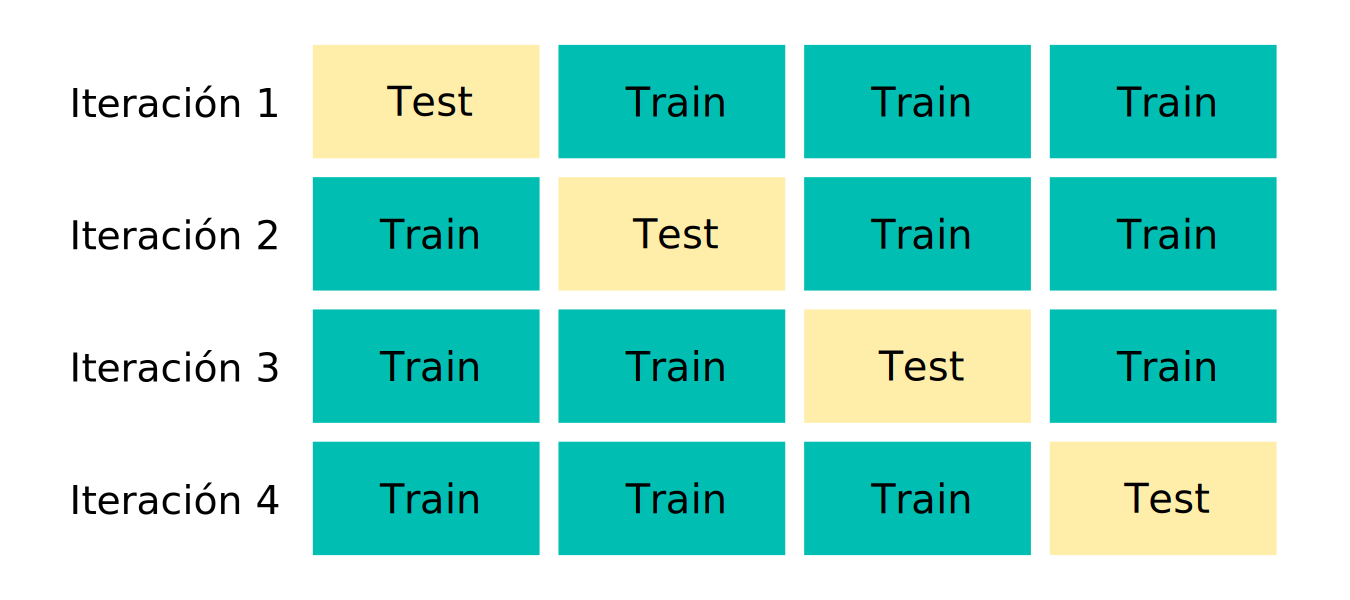
\includegraphics[width=12cm]{figs/KFold_explanation.png}
    \end{center}
\end{figure}

\note[item]{En cuanto al entrenamiento se ha usado la técnica de validación cruzada K-Fold de 4 pliegues stratificada. Se ha hecho esto porque como el dataset tiene muy pocas muestras, pues de esta manera se consiguen usar todos los datos como entrenamiento y todos los datos como prueba y así generalizar al máximo los modelos sin sobreentrenarlos.}

\note[item]{Esta técnica se ha usado para buscar los parámetros óptimos de cada algoritmo y luego también se ha usado para comprobar la preción en el entrenamiento.}
\end{frame}

\begin{frame}{Búsqueda de los parámetros óptimos}
    \begin{figure}
    \begin{center}
        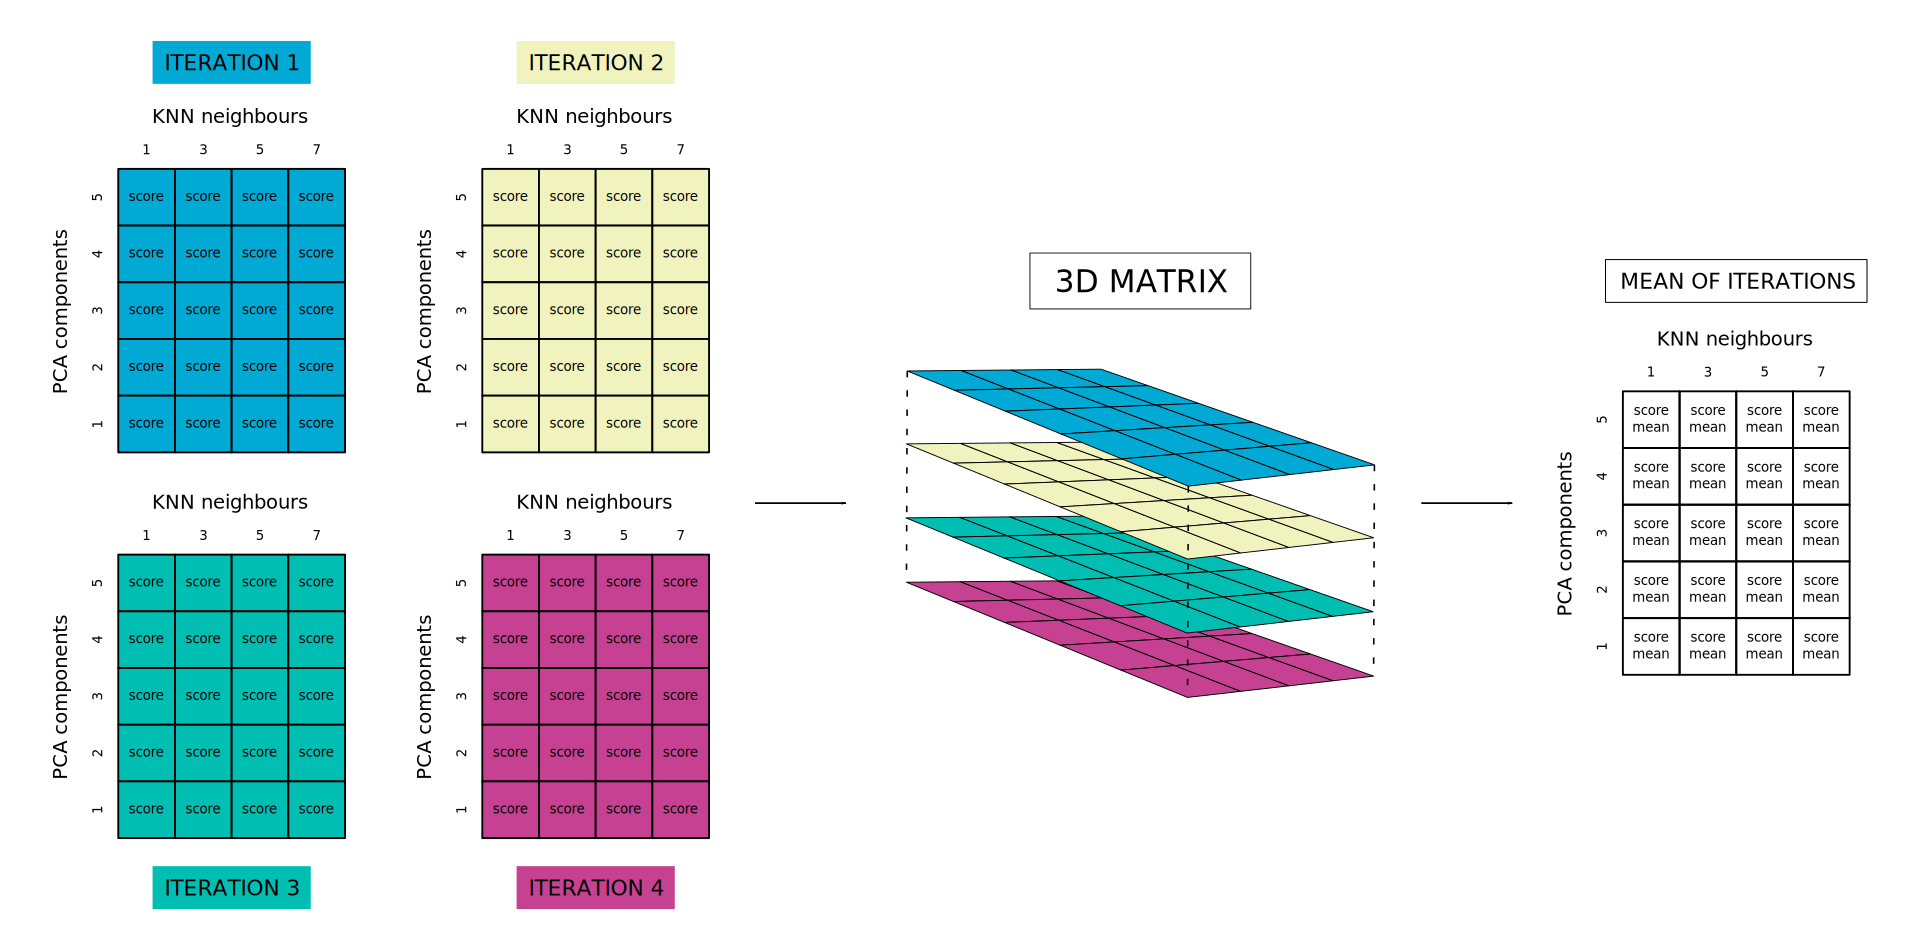
\includegraphics[width=12cm]{figs/KFold_KNN_PCA.png}
    \end{center}
\end{figure}
\end{frame}

\begin{frame}{Parámetros óptimos}
\begin{block}{Intervalos de valores testeados}
\begin{itemize}
    \item PCA: número de \textit{componentes} en [2, 20]
    \item KNN: valores impares de \textit{k} en [1, 13]
    \item SVM: valores de \textit{C} en [1, 999] con saltos de 10
    \item MLP: 1 capa oculta de [5, 24] \textit{neuronas}
\end{itemize}
\end{block}

\begin{table}[H]
\begin{center}
\begin{tabular}{|c|c|}
    \hline
    \textbf{Clasificador y PCA} & \textbf{Parámetros} \\
    \hline
     KNN y PCA & k = 7, n\_components = 11\\
     SVM y PCA & C = 21, n\_components = 11\\
     MLP y PCA & hidden\_layer\_sizes = (17), n\_components = 11\\
     \hline
 \end{tabular}
\end{center}
\end{table}
\end{frame}

\begin{frame}{Resultados del entrenamiento}
\label{diapo:resultados_entrenamiento}
\begin{table}[H]
\begin{center}
\begin{tabular}{|c|c|c|c|c|}
     \hline
    \textbf{Clasificador} & \textbf{Accuracy} & \textbf{Precision} & \textbf{Recall} & \textbf{F1-score}\\
    \hline
     KNN & 0.95 & 0.93 & 0.94 & 0.92\\
     SVM & 0.95 & 0.93 & 0.92 & 0.92\\
     MLP & 0.95 & 0.95 & 0.93 & 0.93\\
     \hline
\end{tabular}
\end{center}
\end{table}
\end{frame}

\subsection{Funcionamiento del sistema}
\begin{frame}{Esquema de funcionamiento del sistema}
\begin{figure}
    \begin{center}
        \includegraphics[width=11cm]{figs/func.png}
    \end{center}
\end{figure}
\end{frame}

\subsection{Integración en ROS}
\begin{frame}{Esquema de funcionamiento del sistema en ROS}
\begin{figure}
    \begin{center}
        \includegraphics[width=12cm]{figs/paquete_ros.png}
    \end{center}
\end{figure}
\end{frame}

\begin{frame}{Parámetros de configuración}
\begin{figure}
  \centering
  \includegraphics[width=12cm]{figs/yamls.png}
\end{figure}
\end{frame}

\subsection{Uso y rendimiento}
\begin{frame}{Ejemplo de funcionamiento con 1 cara}
\begin{figure}[h!]
  \begin{center}
    \subcapcentertrue
    \subfigure{\includegraphics[width=45mm]{figs/prediccion_happy.png}}
    \subfigure{\includegraphics[width=45mm]{figs/prediccion_anger.png}}
    \subfigure{\includegraphics[width=45mm]{figs/prediccion_sadness.png}}
    \subfigure{\includegraphics[width=45mm]{figs/prediccion_surprise.png}}
  \end{center}
\end{figure}
\end{frame}

\begin{frame}{Ejemplo de funcionamiento con 2 caras}
\begin{figure}[h!]
  \begin{center}
    \subcapcentertrue
    \subfigure{\includegraphics[width=45mm]{figs/prediccion_happy_surprise.png}}
    \subfigure{\includegraphics[width=80mm]{figs/salida_topic.png}}
  \end{center}
\end{figure}
\end{frame}

\begin{frame}{Rendimiento}
\begin{block}{max\_num\_faces: 1}
\begin{table}[H]
\begin{center}
\begin{adjustbox}{max width=\textwidth}
\begin{tabular}{|c|c|c|c|}
     \hline
    \textbf{Caras detectadas} & \textbf{Media de FPS} & \textbf{Valor máximo de FPS} & \textbf{Valor mínimo de FPS}\\
    \hline
     1 & 13.18 & 15.13 & 11.04\\
     \hline
 \end{tabular}
 \end{adjustbox}
\end{center}
\end{table}
\end{block}

\begin{block}{max\_num\_faces: 2}
\begin{table}[H]
\begin{center}
\begin{adjustbox}{max width=\textwidth}
\begin{tabular}{|c|c|c|c|}
     \hline
    \textbf{Caras detectadas} & \textbf{Media de FPS} & \textbf{Valor máximo de FPS} & \textbf{Valor mínimo de FPS}\\
    \hline
     1 & 11.11 & 11.97 & 9.18\\
     2 & 7.53 & 8.35 & 6.96\\
     \hline
 \end{tabular}
 \end{adjustbox}
\end{center}
\end{table}
\end{block}

\begin{block}{max\_num\_faces: 3}
\begin{table}[H]
\begin{center}
\begin{adjustbox}{max width=\textwidth}
\begin{tabular}{|c|c|c|c|}
     \hline
    \textbf{Caras detectadas} & \textbf{Media de FPS} & \textbf{Valor máximo de FPS} & \textbf{Valor mínimo de FPS}\\
    \hline
     1 & 11.05 & 11.72 & 9.41\\
     2 & 6.77 & 7.61 & 6.15\\
     3 & 5.37 & 6.93 & 5.02\\
     \hline
 \end{tabular}
 \end{adjustbox}
\end{center}
\end{table}
\end{block}
\end{frame}

\section*{}
\begin{frame}{}
  \centering \Huge
  \emph{Estudios de optimización}
\end{frame}

\section{Estudios de optimización}
\subsection{Búsqueda del detector de puntos faciales óptimo}
\begin{frame}{Estudio de rendimiento para dlib y MediaPipe}
\begin{figure}[h!]
  \begin{center}
    \includegraphics[width=12cm]{figs/pruebas_rendimiento_puntos.png}
  \end{center}
\end{figure}
\end{frame}

\begin{frame}{Estudio de precisión para dlib y MediaPipe}
\begin{figure}[h!]
  \begin{center}
    \subcapcentertrue
    \subfigure{\includegraphics[width=25mm]{figs/dlib_buena_luz.png}}
    \subfigure{\includegraphics[width=25mm]{figs/dlib_mala_luz.png}}
    \subfigure{\includegraphics[width=25mm]{figs/dlib_cubiertos.png}}
    \subfigure{\includegraphics[width=25mm]{figs/dlib_girados.png}}
  \end{center}
\end{figure}

\begin{figure}[h!]
  \begin{center}
    \subcapcentertrue
    \subfigure{\includegraphics[width=25mm]{figs/mediapipe_buena_luz.png}}
    \subfigure{\includegraphics[width=26mm]{figs/mediapipe_mala_luz.png}}
    \subfigure{\includegraphics[width=25mm]{figs/mediapipe_cubiertos.png}}
    \subfigure{\includegraphics[width=25mm]{figs/mediapipe_girados.png}}
  \end{center}
\end{figure}

\note[item]{dlib: 578 fallos}
\note[item]{mediapipe: 103 fallos}
\end{frame}

\subsection{Cantidad de ángulos a utilizar en el dataset}
\begin{frame}{Estudio de ángulos más influyentes en cada emoción}
\begin{figure}[h!]
  \begin{center}
    \includegraphics[width=7cm]{figs/emotional_mesh_todos_angulos.png}
  \end{center}
\end{figure}

\note[item]{A la hora de buscar la cantidad de ángulos óptima para generar el dataset}
\end{frame}

\begin{frame}{Resultados del estudio de ángulos más influyentes}
\begin{center}
    \begin{figure}[h!]
  \includegraphics[width=11.5cm]{figs/resultados_angulos_influyentes_rojo.png}
\end{figure}
\end{center}
Volver a la diapositiva \ref{diapo:dataset_generado}.
\end{frame}

\begin{frame}{Resultados del estudio de ángulos más influyentes}
\label{diapo:resultados_angulos_influyentes}
\begin{table}[H]
\begin{center}
\begin{tabular}{|c|c|}
     \hline
    \textbf{Emoción} & \textbf{Ángulos influyentes} \\
    \hline
     Sorpresa & 1, 2, 0, 4, 19 \\
     Tristeza & 2, 1, 12, 16, 14 \\
     Felicidad & 4, 2, 18, 12, 8 \\
     Miedo & 2, 4, 6, 1, 14 \\
     Asco & 12, 16, 2, 15, 1 \\
     Enfado & 2, 12, 1, 16, 15 \\
     Desprecio & 2, 1, 4, 0, 19 \\
     \hline
 \end{tabular}
\end{center}
\end{table}
\vspace{0.5cm}
\centering
Ángulos más influyentes: 2, 12, 1, 16, 15, 4, 6, 14, 18, 8, 0 y 19

\note[item]{Enfado y Asco}
\note[item]{Desprecio y Sorpresa}
\end{frame}

\begin{frame}{Estudio de simetría de las emociones}
\begin{figure}[h!]
  \begin{center}
    \includegraphics[width=7cm]{figs/emotional_mesh_2_mitades.png}
  \end{center}
\end{figure}
\end{frame}

\begin{frame}{Resultados del estudio de simetría}
\begin{figure}[h!]
\includegraphics[width=12cm]{figs/resultados_simetria.png}
\end{figure}
\end{frame}

\begin{frame}{Datasets generados tras los estudios}

\begin{figure}[h!]
  \begin{center}
  \includegraphics[width=12cm]{figs/datasets_generados.png}
  \end{center}
\end{figure}

\end{frame}

\subsection{Búsqueda del dataset óptimo para el entrenamiento}
\begin{frame}{Búsqueda del dataset con más rendimiento}
\begin{block}{Resultados entrenamiento dataset1}
\begin{table}[H]
\begin{center}
\begin{tabular}{|c|c|c|c|c|}
     \hline
    \textbf{Clasificador} & \textbf{Accuracy} & \textbf{Precision} & \textbf{Recall} & \textbf{F1-score}\\
    \hline
     KNN & 0.82 & 0.76 & 0.74 & 0.74\\
     SVM & 0.84 & 0.79 & 0.78 & 0.77\\
     MLP & 0.82 & 0.78 & 0.78 & 0.77\\
     \hline
 \end{tabular}
\end{center}
\end{table}
\end{block}

\begin{block}{Resultados entrenamiento dataset2}
\begin{table}[H]
\begin{center}
\begin{tabular}{|c|c|c|c|c|}
     \hline
    \textbf{Clasificador} & \textbf{Accuracy} & \textbf{Precision} & \textbf{Recall} & \textbf{F1-score}\\
    \hline
     KNN & 0.83 & 0.79 & 0.75 & 0.75\\
     SVM & 0.84 & 0.80 & 0.77 & 0.78\\
     MLP & 0.84 & 0.81 & 0.80 & 0.80\\
     \hline
 \end{tabular}
\end{center}
\end{table}
\end{block}
\end{frame}

\begin{frame}{Entrenamiento con SVM. Iteraciones de K-Fold, dataset2}
    \begin{table}[h!]
\begin{minipage}{0.48\linewidth}
\centering
\begin{adjustbox}{max width=\textwidth}
\begin{tabular}{|c|c|c|c|}
\hline
\textbf{Clase} & \textbf{Precision} & \textbf{Recall} & \textbf{F1-score}\\
\hline
     Enfado & 0.67 & 0.50 & 0.57\\
     Desprecio & 0.67 & 0.50 & 0.57\\
     Asco & 0.76 & 0.87 & 0.81\\
     Miedo & 0.67 & 1.00 & 0.80\\
     Felicidad & 0.94 & 0.94 & 0.94\\
     Tristeza & 0.83 & 0.71 & 0.77\\
     Sorpresa & 0.95 & 0.95 & 0.95\\
\hline
\end{tabular}
\end{adjustbox}
\vspace{0.4cm}

\begin{adjustbox}{max width=\textwidth}
\begin{tabular}{|c|c|c|c|}
\hline
\textbf{Clase} & \textbf{Precision} & \textbf{Recall} & \textbf{F1-score}\\
\hline
     Enfado & 0.75 & 0.82 & 0.78\\
     Desprecio & 0.67 & 0.80 & 0.73\\
     Asco & 0.82 & 0.93 & 0.87\\
     Miedo & 0.80 & 0.67 & 0.73\\
     Felicidad & 0.94 & 0.94 & 0.94\\
     Tristeza & 1.00 & 0.57 & 0.73\\
     Sorpresa & 0.95 & 0.95 & 0.95\\
\hline
\end{tabular}
\end{adjustbox}
\end{minipage}\hfill
\begin{minipage}{0.48\linewidth}
\centering
\begin{adjustbox}{max width=\textwidth}
\begin{tabular}{|c|c|c|c|}
\hline
\textbf{Clase} & \textbf{Precision} & \textbf{Recall} & \textbf{F1-score}\\
\hline
     Enfado & 0.71 & 0.45 & 0.56\\
     Desprecio & 0.57 & 0.80 & 0.67\\
     Asco & 0.76 & 0.93 & 0.84\\
     Miedo & 1.00 & 0.71 & 0.83\\
     Felicidad & 0.85 & 1.00 & 0.92\\
     Tristeza & 0.83 & 0.71 & 0.77\\
     Sorpresa & 1.00 & 0.95 & 0.98\\
\hline
\end{tabular}
\end{adjustbox}
\vspace{0.4cm}

\begin{adjustbox}{max width=\textwidth}
\begin{tabular}{|c|c|c|c|}
\hline
\textbf{Clase} & \textbf{Precision} & \textbf{Recall} & \textbf{F1-score}\\
\hline
     Enfado & 0.67 & 0.55 & 0.60\\
     Desprecio & 0.50 & 0.25 & 0.33\\
     Asco & 0.67 & 0.80 & 0.73\\
     Miedo & 1.00 & 0.67 & 0.80\\
     Felicidad & 1.00 & 1.00 & 1.00\\
     Tristeza & 0.50 & 0.71 & 0.59\\
     Sorpresa & 1.00 & 1.00 & 1.00\\
\hline
\end{tabular}
\end{adjustbox}
\end{minipage}
\end{table}

Volver a la diapositiva \ref{diapo:resultados_angulos_influyentes}.
\end{frame}

\section*{}
\begin{frame}{}
  \centering \Huge
  \emph{Conclusiones}
\end{frame}

\section{Conclusiones}
\begin{frame}
\label{diapo:conclusiones}
\begin{block}{Objetivo principal cumplido}
Reconocimiento de emociones en un sistema de bajo coste.
\end{block}

\begin{block}{Subobjetivos cumplidos}
\begin{itemize}
    \item Estudiar el estado del arte y elegir la técnica más óptima.
    \item Optimizar y adaptar la técnica escogida en nuestra plataforma.
    \item Generar un dataset de valor.
    \item Realizar el entrenamiento del modelo.
    \item Integrar el sistema en ROS.
\end{itemize}
\end{block}

\note[item]{Desarrollar una herramienta de reconocimiento de emociones que sea capaz de funcionar en un sistema robótico de bajo coste bajo el entorno ROS.}
\end{frame}

\begin{frame}
\begin{block}{Líneas futuras}
\begin{itemize}
\item Implementar aplicaciones de HRI que se ayuden de esta herramienta.
\item Portar el sistema a otras plataformas.
\item Añadir nuevas funcionalidades a la herramienta.
\end{itemize}
\end{block}
\vspace{0.5cm}
\begin{figure}
  \begin{center}
    \subfigure{\includegraphics[width=59mm]{figs/hri_abuelo.jpg}}
    \subfigure{\includegraphics[width=52mm]{figs/hri_niños.jpg}}
  \end{center}
\end{figure}
\end{frame}

\begin{frame}[plain]
\large{\titlepage}
\note[item]{Y hasta aquí mi exposición.}
\note[item]{Quedo a disposición del tribunal...}
\end{frame}

\end{document}
